\documentclass[12pt]{article}

\usepackage[portuguese]{babel}
\usepackage[utf8]{inputenc}
\usepackage{amsmath}
\usepackage{commath}
\usepackage[alf]{abntex2cite}
\usepackage{indentfirst}
\usepackage{graphicx}
\usepackage{multicol,lipsum}
\usepackage{subfig}
\usepackage{geometry}
\usepackage[alf]{abntex2cite}


\geometry{
	paper = a4paper,
    inner = 3cm,
    outer = 3cm,
    top = 2cm,
    bottom = 2cm
}

\begin{document}
%\maketitle

\onehalfspacing

\begin{titlepage}
	\begin{center}

		\Huge{Universidade Federal de Alagoas}\\
		\large{Instituto de Computação}\\ 
		\large{Laboratório de Computação Científica e Análise Numérica}\\ 
        \vspace{220pt}
        \textbf{\LARGE{Relatório de acompanhamento de pesquisa}}\\
		%\title{{\large{Título}}}
		\vspace{3,5cm}
	\end{center}
	
	\begin{flushleft}
		\begin{tabbing}
			Aluno: Danilo Fernandes Costa\\
			Professor orientador: Alejandro Frery\\
	\end{tabbing}
 \end{flushleft}
	\vspace{1cm}
	
	\begin{center}
		\vspace{\fill}
			 Dezembro\\
		 2018
			\end{center}
\end{titlepage}

\section{Introdução}

Uma forma interessante de representar-se os dados PolSAR é através da matriz de Kennaugh, visto que é composta apenas por valores reais e preserva a informação de retroespalhamento \cite{ClassificationPolSARGeodesic}. Dada uma matriz de coerência $T$ associada a um pixel da imagem, a sua correspondente matriz de Kennaugh é da forma:

\[K =
\begin{bmatrix}

\frac{ T_{11} + T_{22} + T_{33} }{2} & \Re(T_{12}) & \Re(T_{13}) & \Im(T_{23})\\
\Re(T_{12}) & \frac{T_{11} + T_{22} - T_{33}}{2} & \Re(T_{23}) & \Im(T_{13})\\
\Re(T_{13}) & \Re(T_{23}) & \frac{ T_{11} - T_{22} + T_{33} }{2} & -\Im(T_{12})\\
\Im(T_{23}) & \Im(T_{13}) & -\Im(T_{12}) & \frac{ -T_{11} + T_{22} + T_{33} }{2}\\

\end{bmatrix}
.\]

Dadas as matrizes de Kennaugh $K_1$ e $K_2$, é possível medir a distância entre as mesmas, por meio da distância geodésica, da seguinte forma:
\begin{displaymath}
GD(K_1, K_2) = \frac{2}{\pi} \cos^{-1} \left(\frac{Tr(K_1^T K_2)}{\sqrt{Tr(K_1^T K_1)} \sqrt{Tr(K_2^T K_2})} \right).
\end{displaymath}.

Em posse disto, é possível medir a semelhança, a qual é dada por $f(K_1, K_2) = 1 - GD(K_1, K_2)$, entre os dados PolSAR e retroespalhadores prototípicos conhecidos. Dentre estes, temos o \textit{trihedral}, \textit{dihedral}, \textit{random volume}, \textit{narrow dihedral}, \textit{cylinder}, \textit{dipole}, \textit{left helix}, \textit{right helix}, \textit{+1/4-wave} e \textit{-1/4-wave}, cujas matrizes de Kennaugh são, respectivamente:

\[K_a =
\begin{pmatrix}
1 & 0 & 0 & 0\\
0 & 1 & 0 & 0\\
0 & 0 & 1 & 0\\
0 & 0 & 0 & -1\\
\end{pmatrix},
K_b =
\begin{pmatrix}
1 & 0 & 0 & 0\\
0 & 1 & 0 & 0\\
0 & 0 & -1 & 0\\
0 & 0 & 0 & 1\\
\end{pmatrix},
K_{rv} =
\begin{pmatrix}
1 & 0 & 0 & 0\\
0 & 1/2 & 0 & 0\\
0 & 0 & 1/2 & 0\\
0 & 0 & 0 & 0\\
\end{pmatrix}
.\]

\[K_{nd} =
\begin{pmatrix}
5/8 & 3/8 & 0 & 0\\
3/8 & 5/8 & 0 & 0\\
0 & 0 & -1/2 & 0\\
0 & 0 & 0 & 1/2
\end{pmatrix},
K_{c} =
\begin{pmatrix}
5/8 & 3/8 & 0 & 0\\
3/8 & 5/8 & 0 & 0\\
0 & 0 & 1/2 & 0\\
0 & 0 & 0 & -1/2\\
\end{pmatrix}
,\]

\[K_d=
\begin{pmatrix}
1 & -1 & 0 & 0\\
-1 & 1 & 0 & 0\\
0 & 0 & 0 & 0\\
0 & 0 & 0 & 0\\
\end{pmatrix},
K_{lh}=
\begin{pmatrix}
1 & 0 & 0 & -1\\
0 & 0 & 0 & 0\\
0 & 0 & 0 & 0\\
-1 & 0 & 0 & 1\\
\end{pmatrix},
K_{rh}=
\begin{pmatrix}
1 & 0 & 0 & 1\\
0 & 0 & 0 & 0\\
0 & 0 & 0 & 0\\
1 & 0 & 0 & 1\\
\end{pmatrix}
,\]

\[K_{+1/4}=
\begin{pmatrix}
1 & 0 & 0 & 0\\
0 & 1 & 0 & 0\\
0 & 0 & 0 & 1\\
0 & 0 & 1 & 0\\
\end{pmatrix},
K_{-1/4}=
\begin{pmatrix}
1 & 0 & 0 & 0\\
0 & 1 & 0 & 0\\
0 & 0 & 0 & -1\\
0 & 0 & -1 & 0\\
\end{pmatrix}
.\]

No presente relatório são apresentados histogramas das similaridades dos dados de regiões de vegetação e solo exposto em relação aos retroespalhadores prototípicos supracitados. Os dados utilizados foram obtidos em UAVSAR e referem-se às regiões de Sierra del Lacandon National Park, Guatemala; Ponderosa Forest, Califórnia, EUA e Slumgullion, Colorado, EUA.

\section{Histogramas das similaridades}

Para o cálculo das similaridades é necessário que os dados referentes às bandas HHHH, HVHV, VVVV, HHHV, HHVV e HVVV estejam carregados no formato de matrizes na memória. Feito isto, é calculado a intensidade dos dados complexos referentes a esses três últimos obtendo-se seu módulo por meio da função nativa \texttt{Mod} e elevando o resultado ao quadrado. 

Para calcular as similaridades, executou-se o seguinte script:
\begin{verbatim}
mod_kennaugh <- sqrt( hhhh^2 + hvhv^2 + vvvv^2 + 
                      2*int_hhhv + 2*int_hhvv + 2*int_hvvv )

similarity_trihedral <- 1 - (2/pi)*acos( hhhh / mod_kennaugh )
similarity_dihedral  <- 1 - (2/pi)*acos( hvhv / mod_kennaugh )
similarity_rand_vol  <- 1 - (2/pi)*acos( ( 2*hhhh + hvhv + vvvv ) / 
                                         ( sqrt(6)*mod_kennaugh ) )
                                         
similarity_narrow_dihedral <- 1 - (2/pi)*acos((hhhh + 9*hvhv + 6*Re(hhhv))/
                                                (10*sqrt_trace_kennaugh) )

similarity_cylinder <- 1 - (2/pi)*acos( ( 9*hhhh + hvhv + 6*Re(hhhv) ) /
                                        (10*sqrt_trace_kennaugh) )

similarity_dipole <- 1 - (2/pi)*acos( ( hhhh + hvhv - 2*Re(hhhv) ) /
                                        (2*sqrt_trace_kennaugh) )

similarity_left_helix <- 1 - (2/pi)*acos( ( hvhv + vvvv - 2*Im(hvvv) ) /
                                            (2*sqrt_trace_kennaugh) )
similarity_right_helix <- 1 - (2/pi)*acos( ( hvhv + vvvv + 2*Im(hvvv) ) /
                                            (2*sqrt_trace_kennaugh) )

similarity_pos_wave <- 1 - (2/pi)*acos( ( hhhh + hvhv - 2*Im(hhhv) ) /
                                        (2*sqrt_trace_kennaugh) )
similarity_neg_wave <- 1 - (2/pi)*acos( ( hhhh + hvhv + 2*Im(hhhv) ) /
                                        (2*sqrt_trace_kennaugh) )
\end{verbatim}

Nas figuras \ref{fig:img1}, \ref{fig:img2} e \ref{fig:img3} estão indicadas as regiões cujos dados foram utilizados no cálculo das similaridades em relação aos retroespalhores citados.

\begin{figure}[!h]
    \centering
    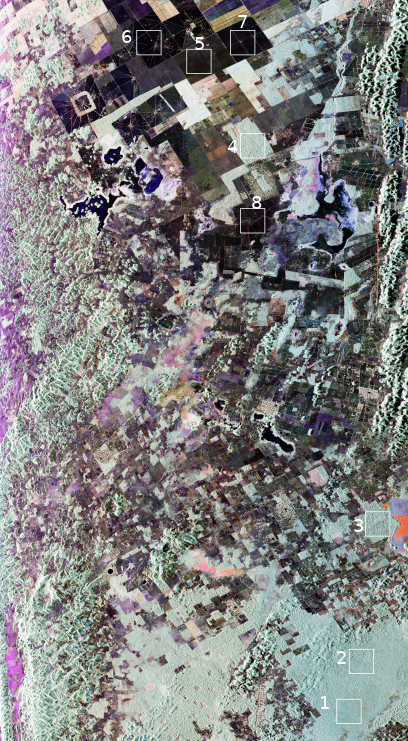
\includegraphics[width = 0.9\linewidth]{../../Images/Report_18_12_20/guatemala.png}
    \caption{Regiões 1, 2, 3, 4 e 5 selecionadas da Sierra del Lacandon National Park, Guatemala}
    \label{fig:img1}
\end{figure}

\begin{figure}[!h]
    \centering
    \includegraphics[width = 0.9\linewidth]{../../Images/Report_18_12_20/ponder.png}
    \caption{Regiões 1, 2, 3 e 4 selecionadas de Ponderosa Forest, California, USA}
    \label{fig:img2}
\end{figure}

\begin{figure}[!h]
    \centering
    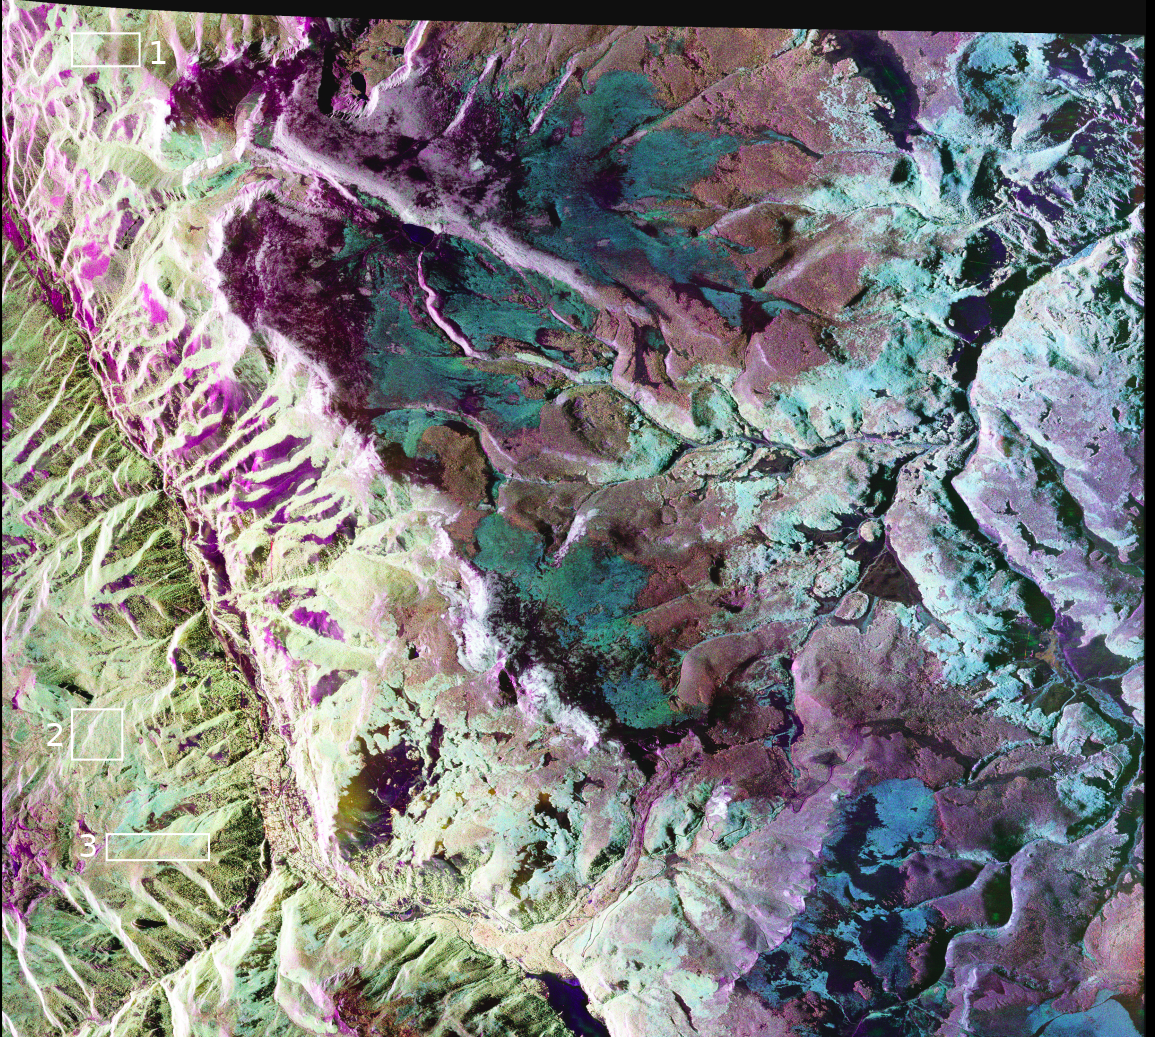
\includegraphics[width = 0.9\linewidth]{../../Images/Report_18_12_20/slum.png}
    \caption{Regiões 1, 2 e 3 selecionadas de Slumgullion, Colorado, USA}
    \label{fig:img3}
\end{figure}
\newpage
As figuras \ref{fig:tri_r1}, \ref{fig:tri_r2}, \ref{fig:tri_r3}, \ref{fig:tri_r4}, \ref{fig:tri_r5}, \ref{fig:pond_tri_r1}, \ref{fig:pond_tri_r2}, \ref{fig:pond_tri_r3}, \ref{fig:pond_tri_r4}, \ref{fig:slum_tri_r1}, \ref{fig:slum_tri_r2} e \ref{fig:slum_tri_r3} apresentam os histogramas das similaridades em relação ao retroespalhador prototípico \textit{trihedral} dos dados de regiões de vegetação com diferentes níveis de cobertura vegetal. Em cada imagem, as regiões selecionadas apresentam nível similar de cobertura vegetal; com execeção da figura \ref{fig:img1}, visto que a região 5 é uma plantação e as regiões 1 à 4 são trechos florestais. É observável o ajuste desses histogramas a distribuições Normais com parâmetros relativamente próximos em regiões de nível similar de vegetação. Além disso, os histogramas sugerem que a diminuição do nível de vegetação implica em um aumento na média e que para valores de média acima de 0.517 começa a apresentar um considerável comportamento assimétrico. Possivelmente, isto se dá devido a detecção de outros retroespalhores, como solo.

\newpage

\begin{figure}[!h]
    \centering
    \vspace{0.1\linewidth}
    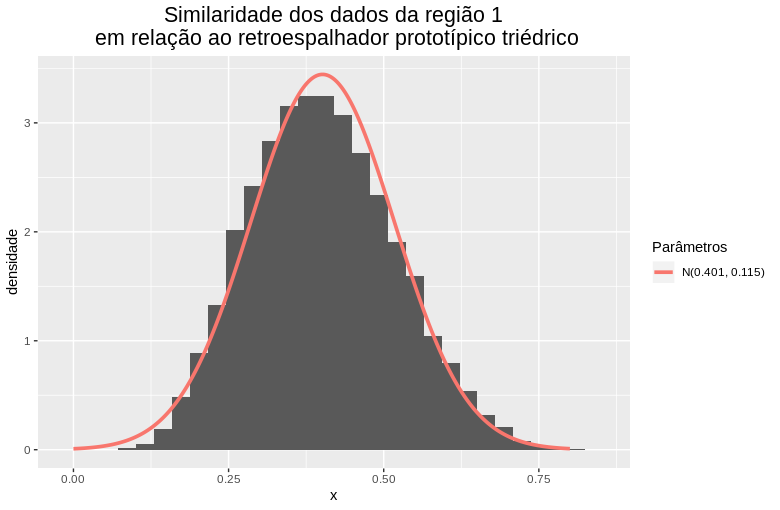
\includegraphics[width = 0.95\linewidth]{../../Images/Report_18_12_17/tri_region1.png}
    \caption{Região 1, Guatemala}
    \label{fig:tri_r1}
\end{figure}

\begin{figure}[!h]
    \centering
    \vspace{0.15\linewidth}
    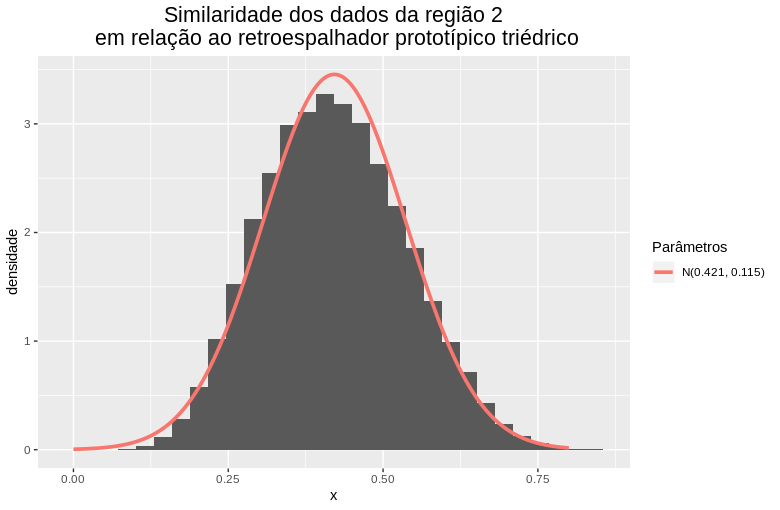
\includegraphics[width = 0.95\linewidth]{../../Images/Report_18_12_17/tri_region2.png}
    \caption{Região 2, Guatemala}
    \label{fig:tri_r2}
\end{figure}

\begin{figure}[!h]
    \centering
    \vspace{0.15\linewidth}
    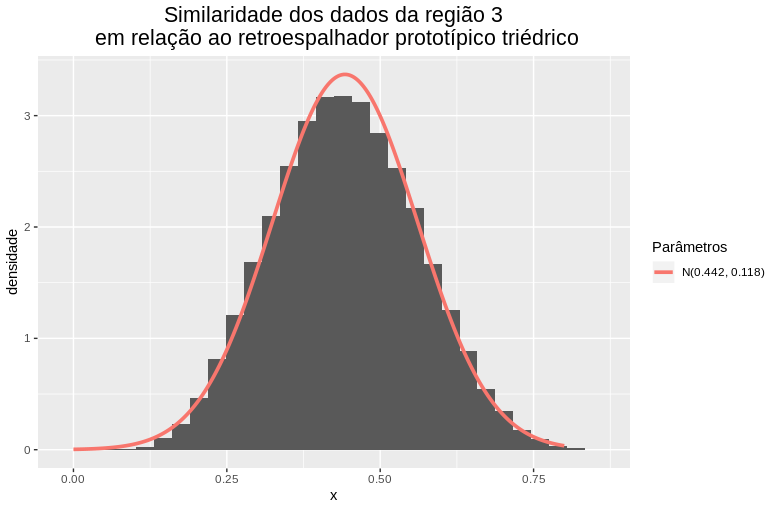
\includegraphics[width = 0.95\linewidth]{../../Images/Report_18_12_17/tri_region3.png}
    \caption{Região 3, Guatemala}
    \label{fig:tri_r3}
\end{figure}

\begin{figure}[!h]
    \centering    
    \vspace{0.1\linewidth}
    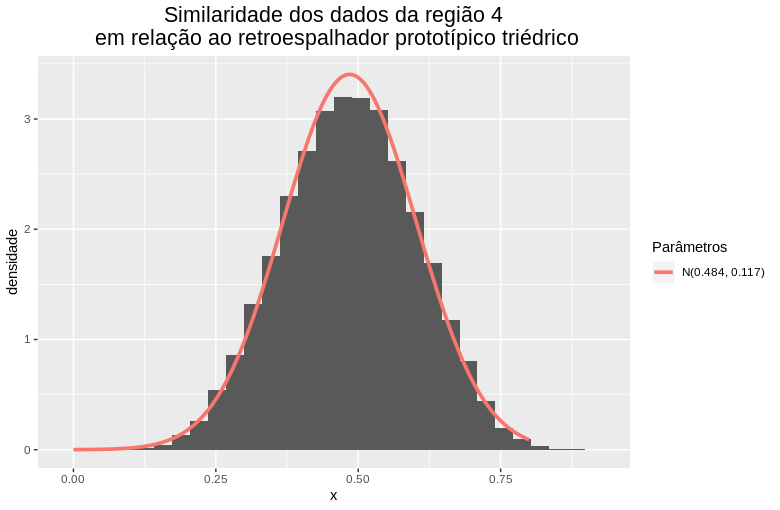
\includegraphics[width = 0.95\linewidth]{../../Images/Report_18_12_17/tri_region4.png}
    \caption{Região 4, Guatemala}
    \label{fig:tri_r4}
\end{figure}

\begin{figure}[!h]
    \centering    
    \vspace{0.1\linewidth}
    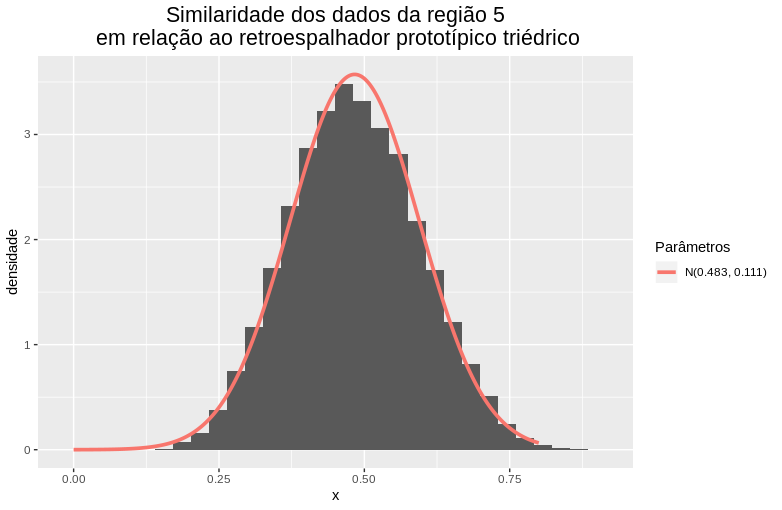
\includegraphics[width = 0.95\linewidth]{../../Images/Report_18_12_17/tri_region5.png}
    \caption{Região 5, Guatemala}
    \label{fig:tri_r5}
\end{figure}

\begin{figure}[!h]
    \centering
    \vspace{0.1\linewidth}
    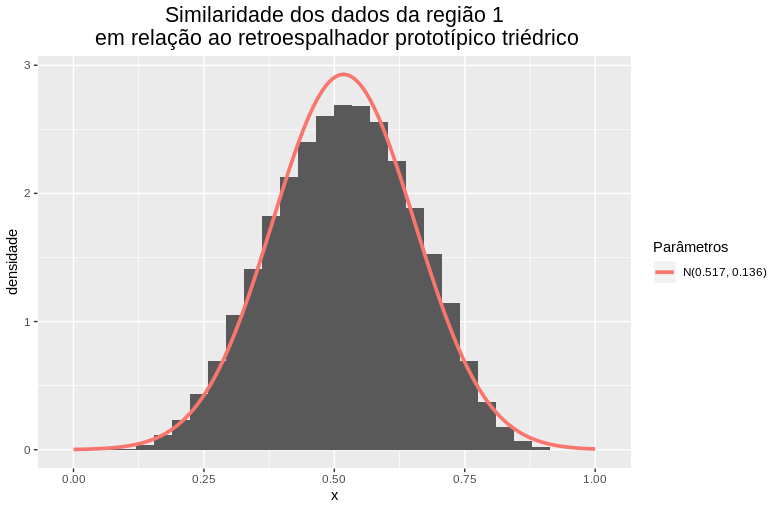
\includegraphics[width = \linewidth]{../../Images/Report_18_12_20/ponder_tri_region1.png}
    \caption{Região 1, Ponderosa Forest}
    \label{fig:pond_tri_r1}
\end{figure}

\begin{figure}[!h]
    \centering
    \vspace{0.1\linewidth}
    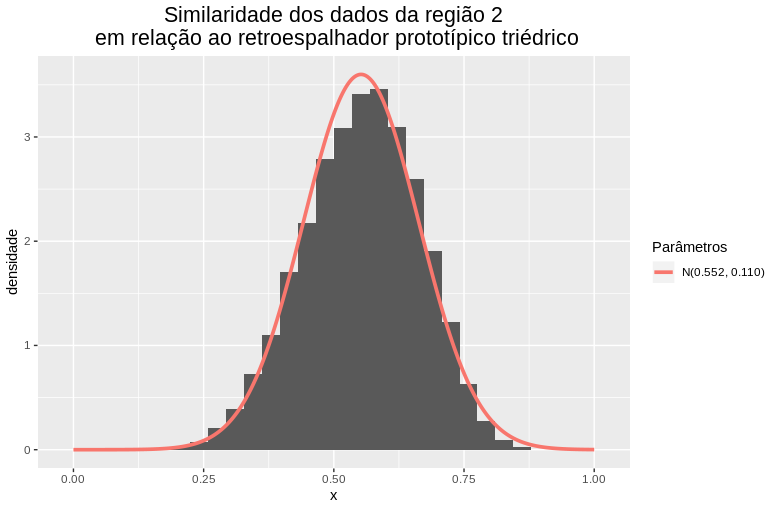
\includegraphics[width = \linewidth]{../../Images/Report_18_12_20/ponder_tri_region2.png}
    \caption{Região 2, Ponderosa Forest}
    \label{fig:pond_tri_r2}
\end{figure}

\begin{figure}[!h]
    \centering
    \vspace{0.1\linewidth}
    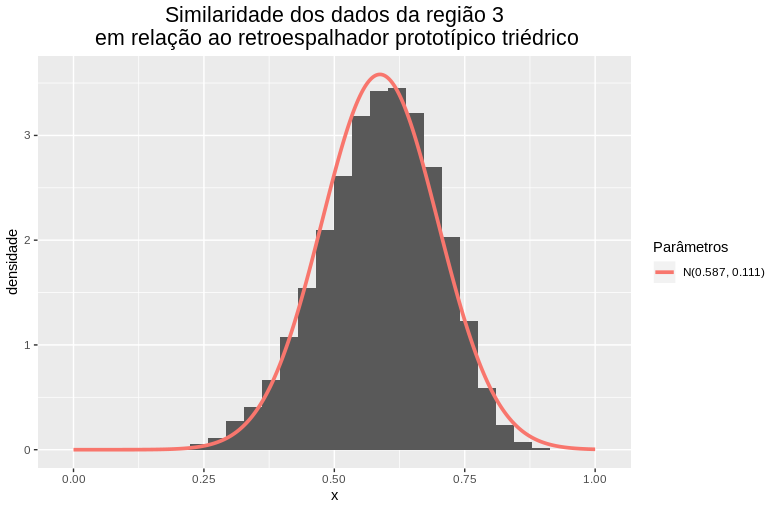
\includegraphics[width = \linewidth]{../../Images/Report_18_12_20/ponder_tri_region3.png}
    \caption{Região 3, Ponderosa Forest}
    \label{fig:pond_tri_r3}
\end{figure}

\begin{figure}[!h]
    \centering
    \vspace{0.1\linewidth}
    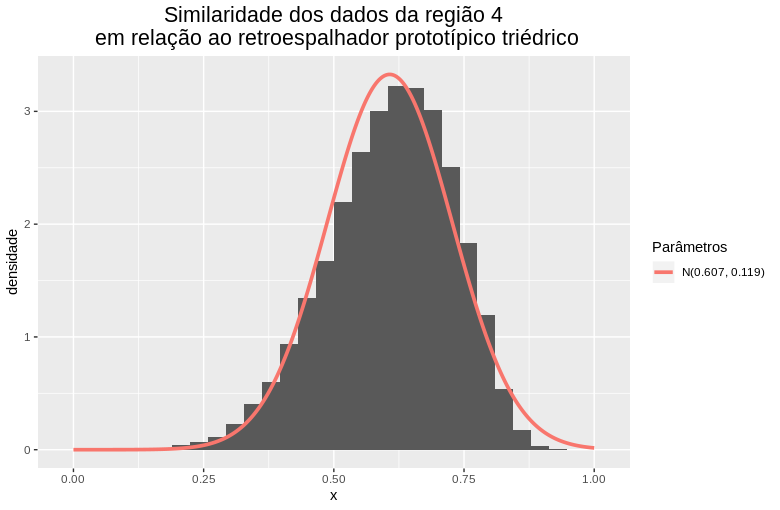
\includegraphics[width = \linewidth]{../../Images/Report_18_12_20/ponder_tri_region4.png}
    \caption{Região 4, Ponderosa Forest}
    \label{fig:pond_tri_r4}
\end{figure}

\begin{figure}[!h]
    \centering
    \vspace{0.1\linewidth}
    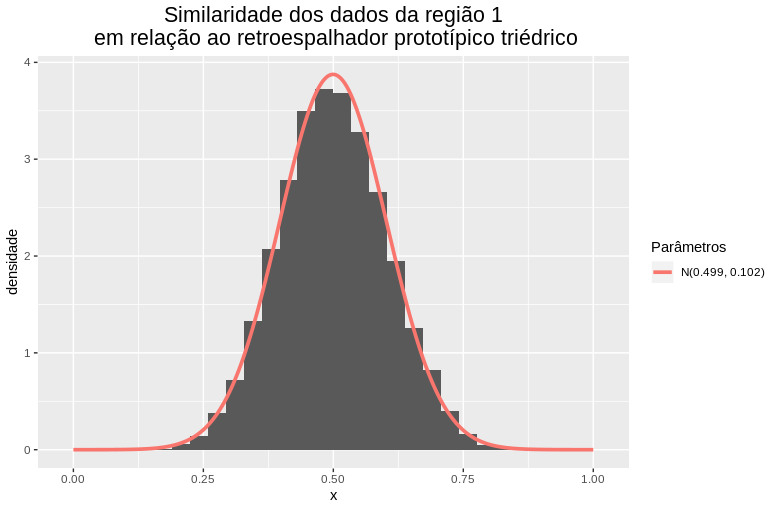
\includegraphics[width = \linewidth]{../../Images/Report_18_12_20/slum_tri_region1.png}
    \caption{Região 1, Slumgullion}
    \label{fig:slum_tri_r1}
\end{figure}

\begin{figure}[!h]
    \centering
    \vspace{0.1\linewidth}
    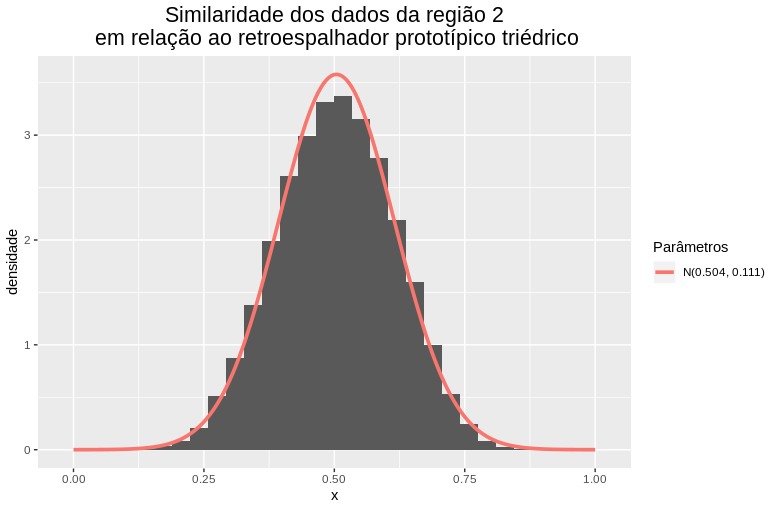
\includegraphics[width = \linewidth]{../../Images/Report_18_12_20/slum_tri_region2.png}
    \caption{Região 2, Slumgullion}
    \label{fig:slum_tri_r2}
\end{figure}

\begin{figure}[!h]
    \centering
    \vspace{0.1\linewidth}
    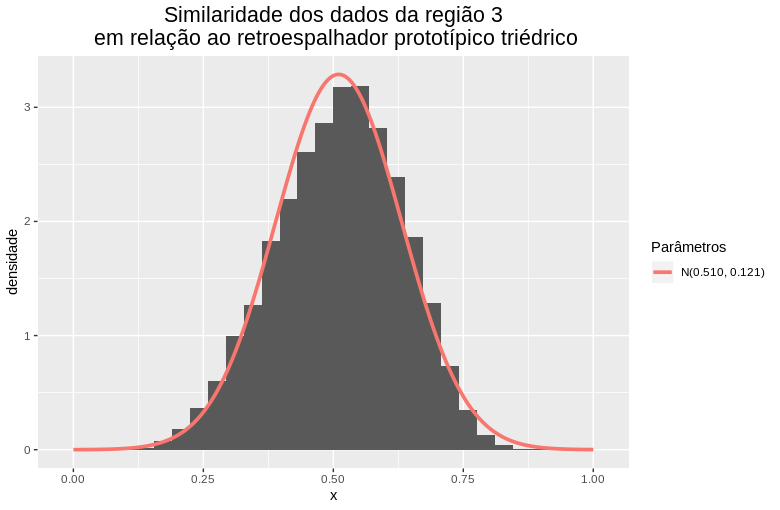
\includegraphics[width = \linewidth]{../../Images/Report_18_12_20/slum_tri_region3.png}
    \caption{Região 3, Slumgullion}
    \label{fig:slum_tri_r3}
\end{figure}


As figuras \ref{fig:di_r1}, \ref{fig:di_r2}, \ref{fig:di_r3}, \ref{fig:di_r4}, \ref{fig:di_r5}, \ref{fig:pond_di_r1}, \ref{fig:pond_di_r2}, \ref{fig:pond_di_r3}, \ref{fig:pond_di_r4},  \ref{fig:slum_di_r1}, \ref{fig:slum_di_r2} e \ref{fig:slum_di_r3} apresentam os histogramas das similaridades em relação ao retroespalhador prototípico \textit{dihedral} dos dados de regiões de vegetação das três imagens. É notório o ajuste dos histogramas a distribuições Gama com parâmetros relativamente próximos, com exceção da figura \ref{fig:di_r5}. Deve ser observado que esses parâmetros foram estimados utilizando a função \texttt{mle} da bilioteca \texttt{stats4}.

\begin{figure}[!h]
    \centering
    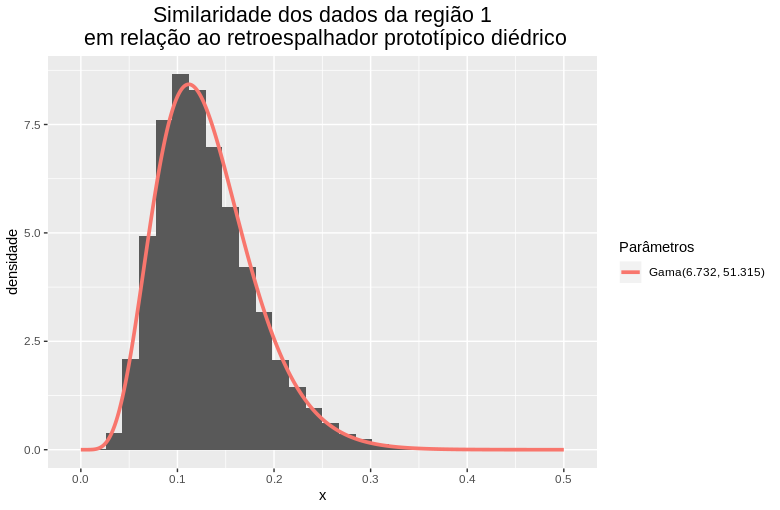
\includegraphics[width = 0.93\linewidth]{../../Images/Report_18_12_17/di_region1.png}
    \caption{Região 1, Guatemala}
    \label{fig:di_r1}
\end{figure}

\begin{figure}[!h]
    \centering
    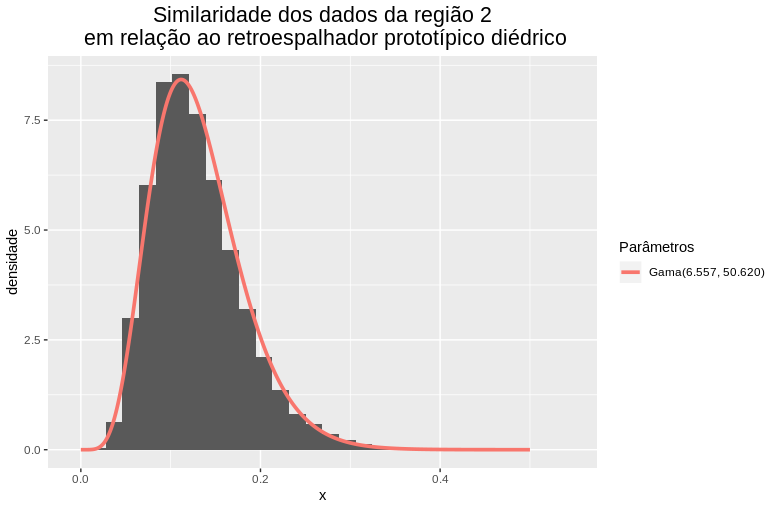
\includegraphics[width = 0.93\linewidth]{../../Images/Report_18_12_17/di_region2.png}
    \caption{Região 2, Guatemala}
    \label{fig:di_r2}
\end{figure}

\begin{figure}[!h]
    \centering
    \vspace{0.1\linewidth}
    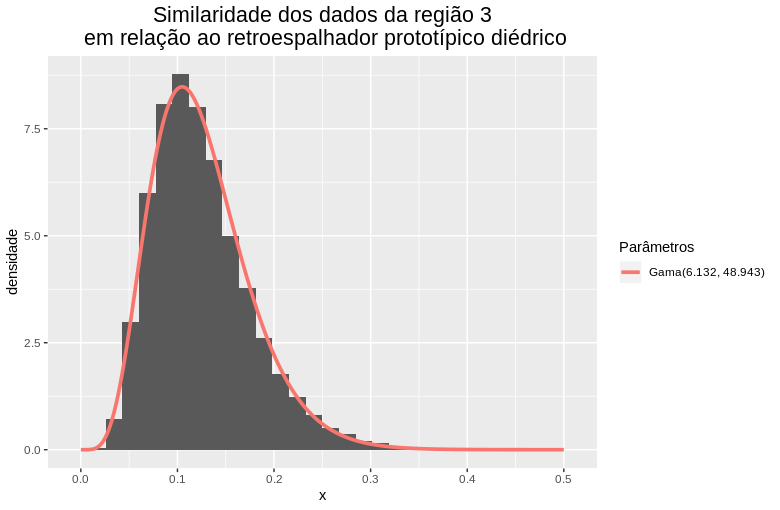
\includegraphics[width = 0.95\linewidth]{../../Images/Report_18_12_17/di_region3.png}
    \caption{Região 3, Guatemala}
    \label{fig:di_r3}
\end{figure}

\begin{figure}[!h]
    \centering
    \vspace{0.15\linewidth}
    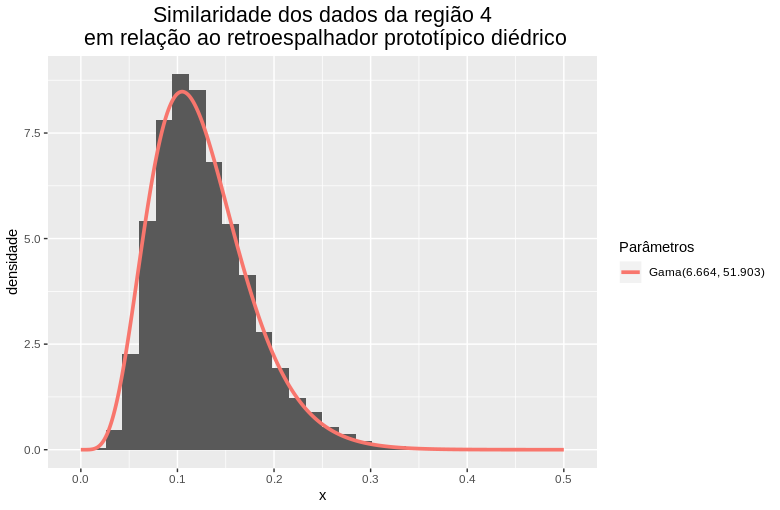
\includegraphics[width = 0.95\linewidth]{../../Images/Report_18_12_17/di_region4.png}
    \caption{Região 4, Guatemala}
    \label{fig:di_r4}
\end{figure}

\begin{figure}[!h]
    \centering
    \vspace{0.1\linewidth}
    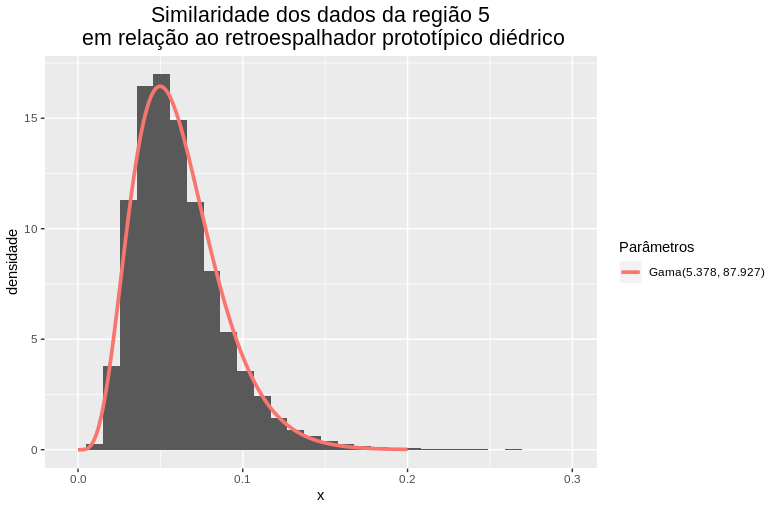
\includegraphics[width = 0.95\linewidth]{../../Images/Report_18_12_17/di_region5.png}
    \caption{Região 5, Guatemala}
    \label{fig:di_r5}
\end{figure}

\begin{figure}[!h]
    \centering
    \vspace{0.1\linewidth}
    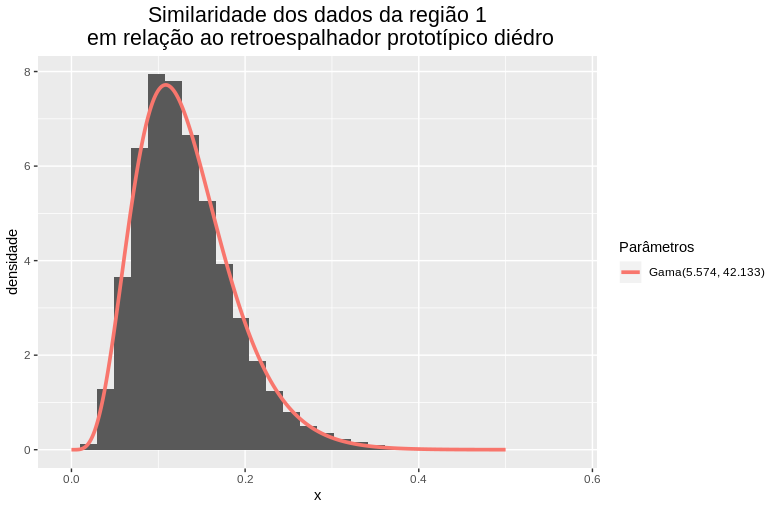
\includegraphics[width = \linewidth]{../../Images/Report_18_12_20/ponder_di_region1.png}
    \caption{Região 1, Ponderosa Forest}
    \label{fig:pond_di_r1}
\end{figure}

\begin{figure}[!h]
    \centering
    \vspace{0.08\linewidth}
    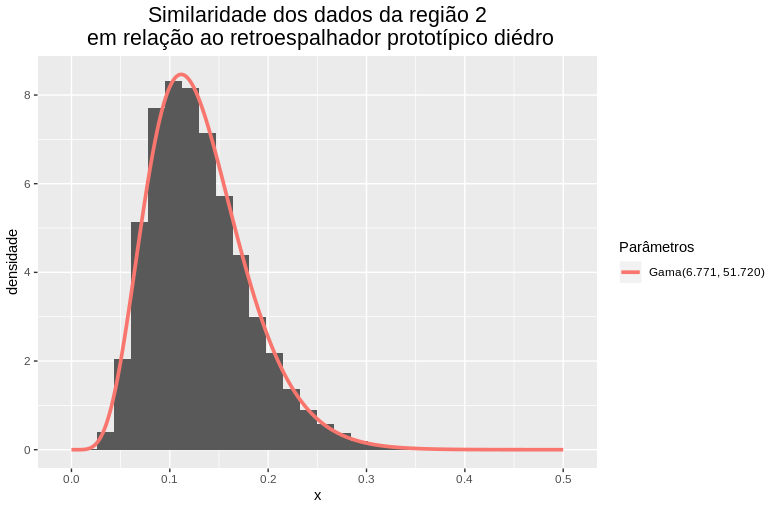
\includegraphics[width = \linewidth]{../../Images/Report_18_12_20/ponder_di_region2.png}
    \caption{Região 2, Ponderosa Forest}
    \label{fig:pond_di_r2}
\end{figure}

\begin{figure}[!h]
    \centering
    \vspace{0.1\linewidth}
    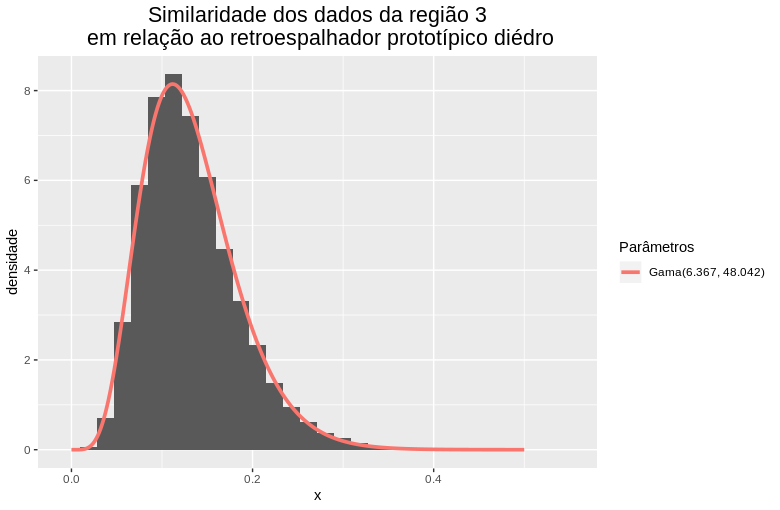
\includegraphics[width = \linewidth]{../../Images/Report_18_12_20/ponder_di_region3.png}
    \caption{Região 3, Ponderosa Forest}
    \label{fig:pond_di_r3}
\end{figure}

\begin{figure}[!h]
    \centering
    \vspace{0.1\linewidth}
    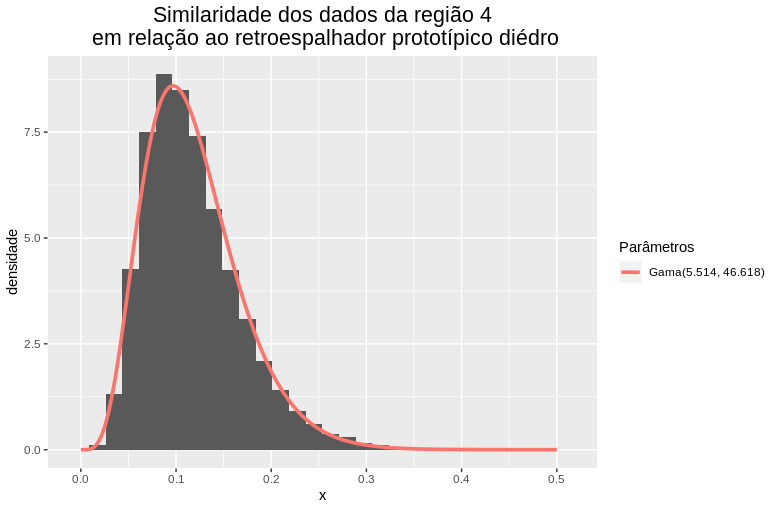
\includegraphics[width = \linewidth]{../../Images/Report_18_12_20/ponder_di_region4.png}
    \caption{Região 4, Ponderosa Forest}
    \label{fig:pond_di_r4}
\end{figure}

\begin{figure}[!h]
    \centering
    \vspace{0.1\linewidth}
    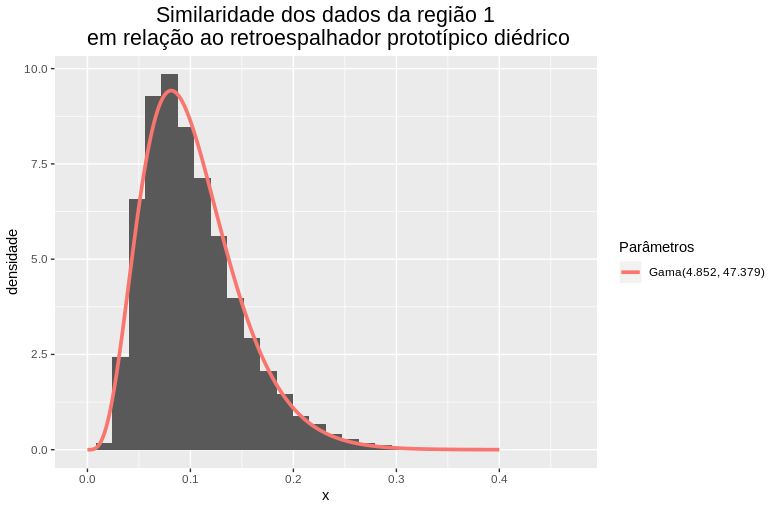
\includegraphics[width = \linewidth]{../../Images/Report_18_12_20/slum_di_region1.png}
    \caption{Região 1, Slumgullion}
    \label{fig:slum_di_r1}
\end{figure}

\begin{figure}[!h]
    \centering
    \vspace{0.1\linewidth}
    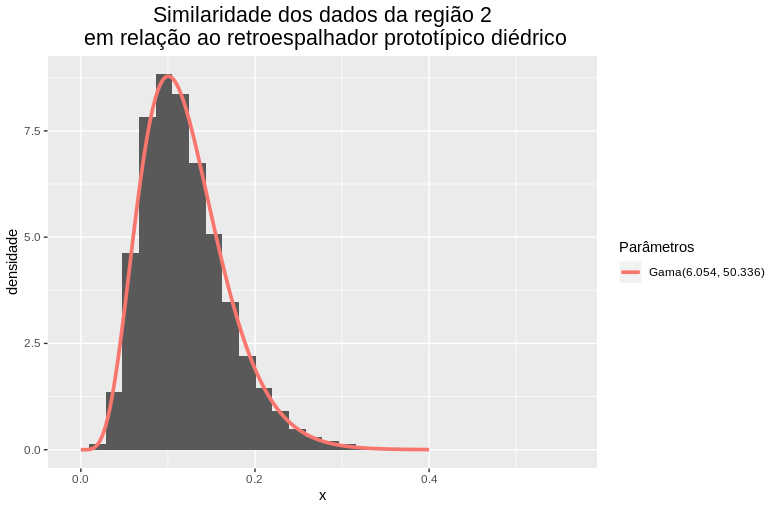
\includegraphics[width = \linewidth]{../../Images/Report_18_12_20/slum_di_region2.png}
    \caption{Região 2, Slumgullion}
    \label{fig:slum_di_r2}
\end{figure}

\begin{figure}[!h]
    \centering
    \vspace{0.1\linewidth}
    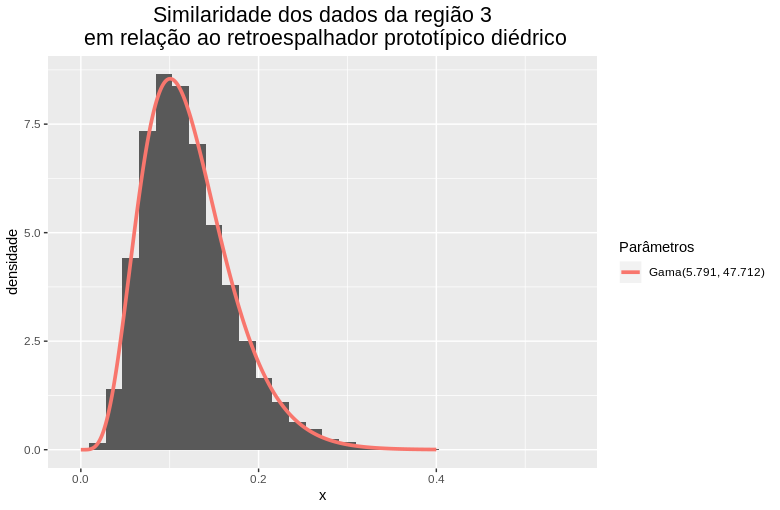
\includegraphics[width = \linewidth]{../../Images/Report_18_12_20/slum_di_region3.png}
    \caption{Região 3, Slumgullion}
    \label{fig:slum_di_r3}
\end{figure}

As figuras \ref{fig:rv_r1}, \ref{fig:rv_r2}, \ref{fig:rv_r3}, \ref{fig:rv_r4}, \ref{fig:rv_r5}, \ref{fig:pond_rv_r1}, \ref{fig:pond_rv_r2}, \ref{fig:pond_rv_r3}, \ref{fig:pond_rv_r4}, \ref{fig:slum_rv_r1}, \ref{fig:slum_rv_r2} e \ref{fig:slum_rv_r3} apresentam os histogramas das similaridades dos dados das regiões de vegetação em relação ao retroespalhador prototípico \textit{random volume}. Novamente, é possível observar o ajuste dos histogramas a distribuições Normais com parâmetros próximos. Além disso, pode ser notado que ocorreu o fenômeno análogo ao que aconteceu nos histogramas que envolviam o retroespalhador \textit{trihedral}

\begin{figure}[!h]
    \centering
    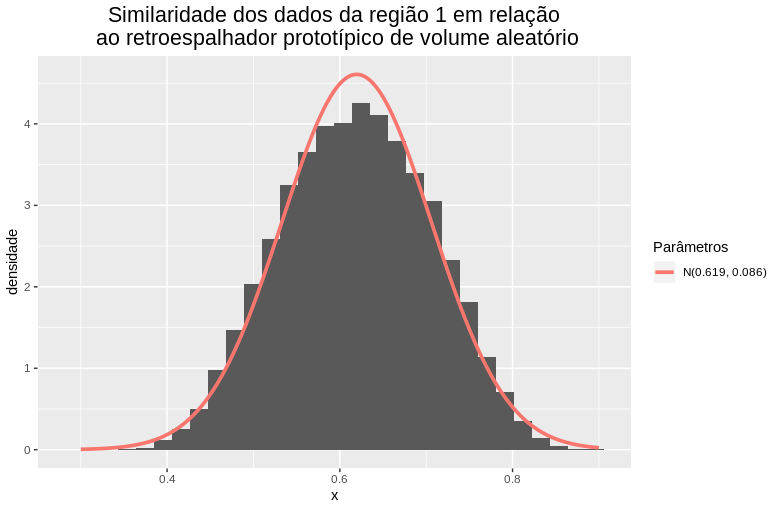
\includegraphics[width = 0.95\linewidth]{../../Images/Report_18_12_17/rv_region1.png}
    \caption{Região 1, Guatemala}
    \label{fig:rv_r1}
\end{figure}

\begin{figure}[!h]
    \centering
    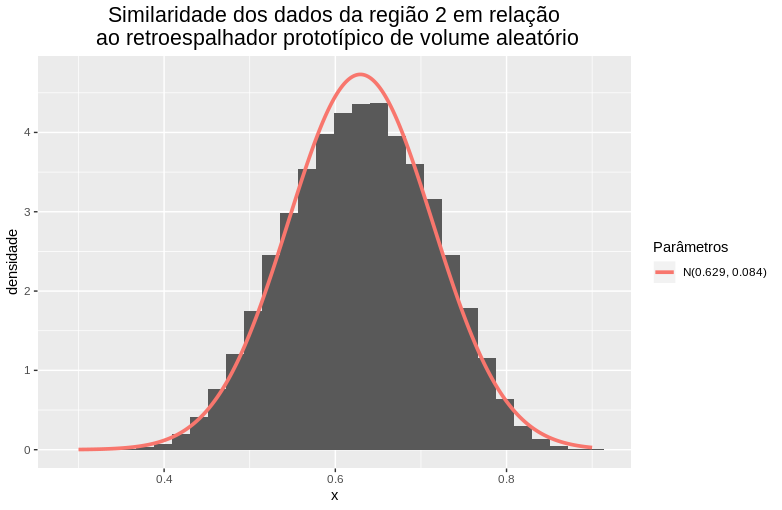
\includegraphics[width = 0.95\linewidth]{../../Images/Report_18_12_17/rv_region2.png}
    \caption{Região 2, Guatemala}
    \label{fig:rv_r2}
\end{figure}

\begin{figure}[!h]
    \centering
    \vspace{0.15\linewidth}
    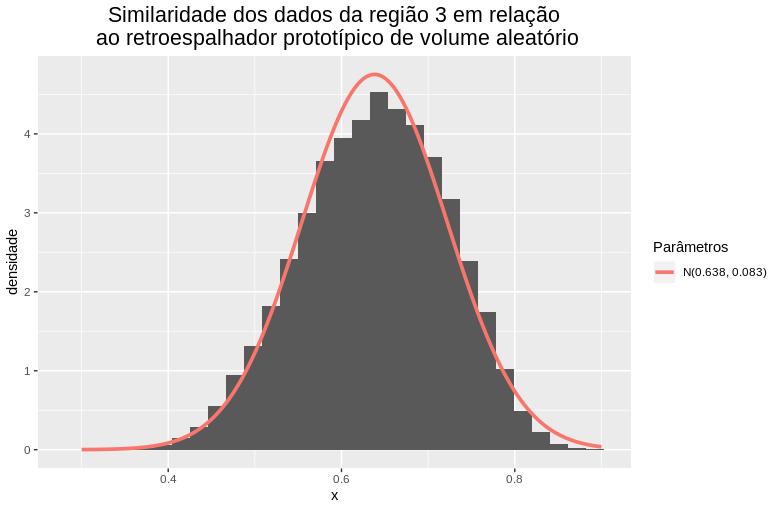
\includegraphics[width = 0.95\linewidth]{../../Images/Report_18_12_17/rv_region3.png}
    \caption{Região 3, Guatemala}
    \label{fig:rv_r3}
\end{figure}

\begin{figure}[!h]
    \centering    
    \vspace{0.1\linewidth}
    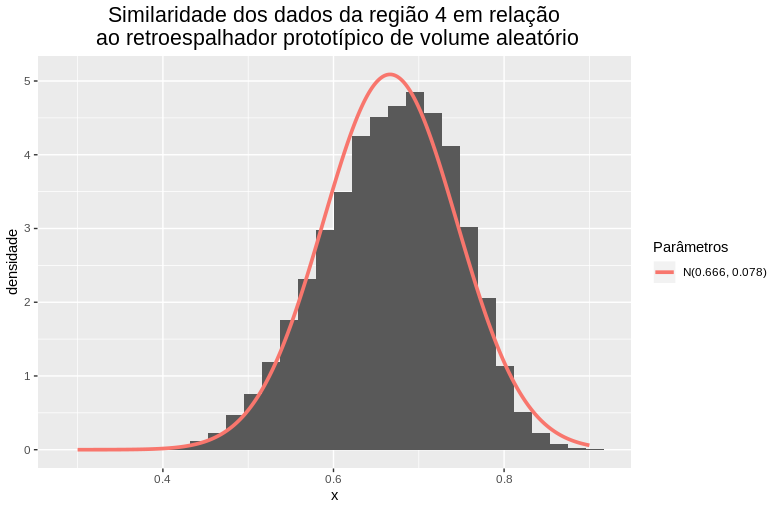
\includegraphics[width = 0.95\linewidth]{../../Images/Report_18_12_17/rv_region4.png}
    \caption{Região 4, Guatemala}
    \label{fig:rv_r4}
\end{figure}

\begin{figure}[!h]
    \centering    
    \vspace{0.1\linewidth}
    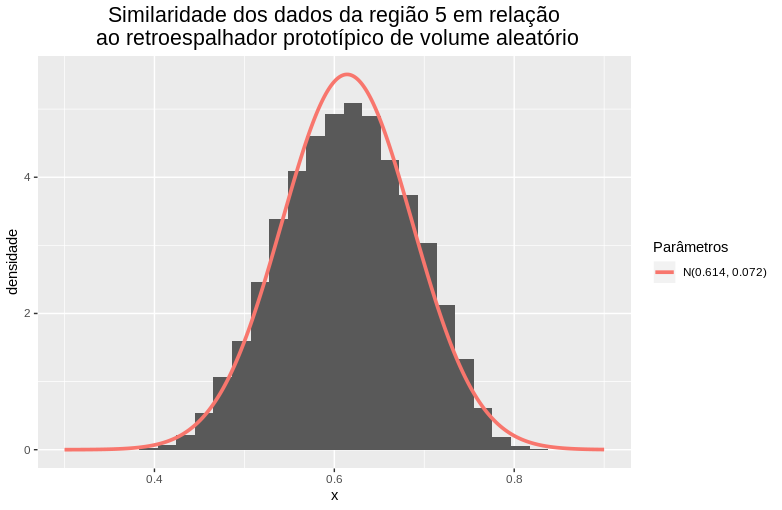
\includegraphics[width = 0.95\linewidth]{../../Images/Report_18_12_17/rv_region5.png}
    \caption{Região 5, Guatemala}
    \label{fig:rv_r5}
\end{figure}

\begin{figure}[!h]
    \centering
    \vspace{0.15\linewidth}
    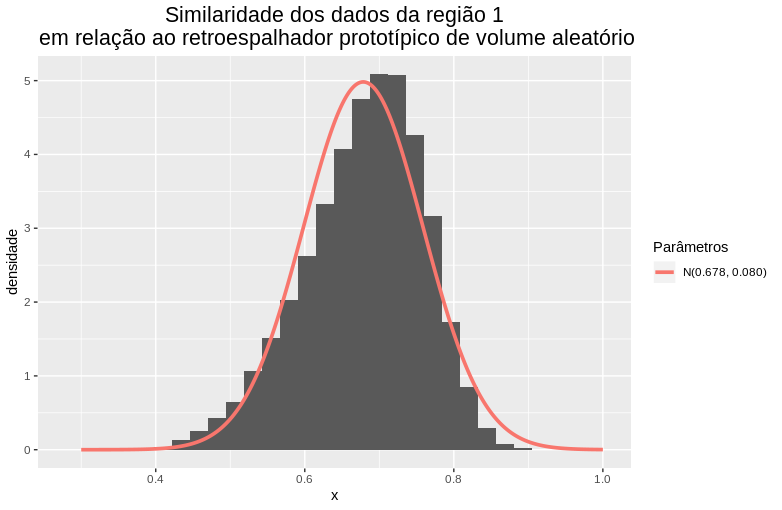
\includegraphics[width = 0.95\linewidth]{../../Images/Report_18_12_20/ponder_rv_region1.png}
    \caption{Região 1, Ponderosa Forest}
    \label{fig:pond_rv_r1}
\end{figure}

\begin{figure}[!h]
    \centering
    \vspace{0.1\linewidth}
    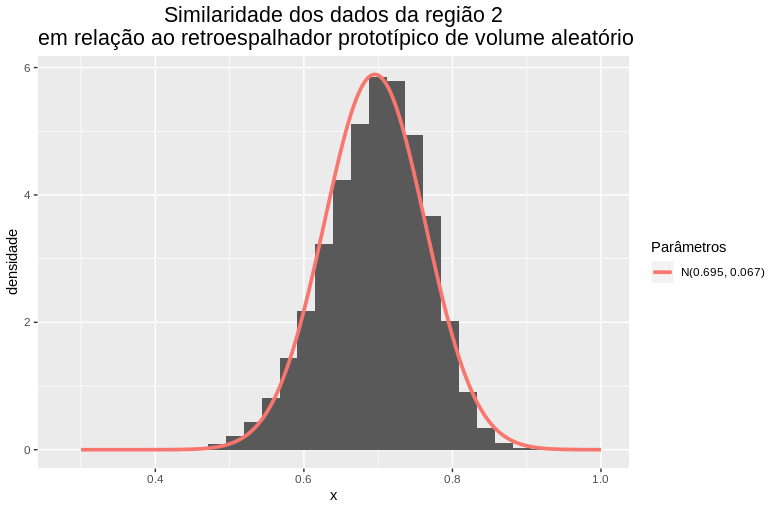
\includegraphics[width = 0.95\linewidth]{../../Images/Report_18_12_20/ponder_rv_region2.png}
    \caption{Região 2, Ponderosa Forest}
    \label{fig:pond_rv_r2}
\end{figure}

\begin{figure}[!h]
    \centering
    \vspace{0.1\linewidth}
    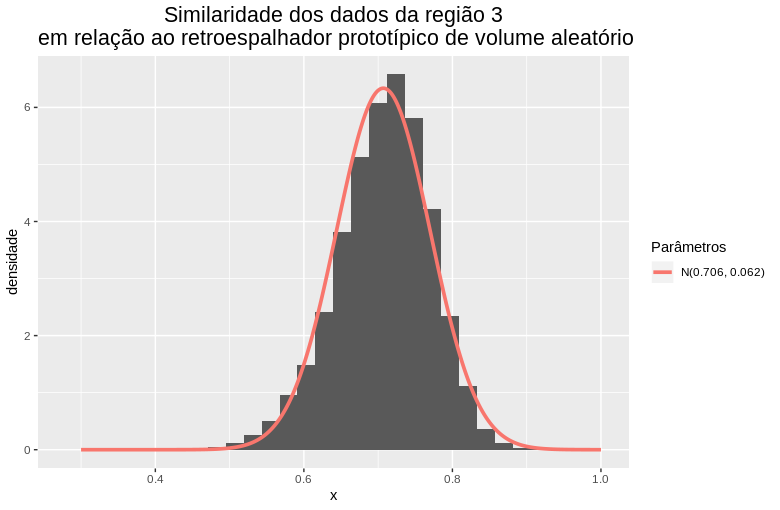
\includegraphics[width = \linewidth]{../../Images/Report_18_12_20/ponder_rv_region3.png}
    \caption{Região 3, Ponderosa Forest}
    \label{fig:pond_rv_r3}
\end{figure}

\begin{figure}[!h]
    \centering
    \vspace{0.1\linewidth}
    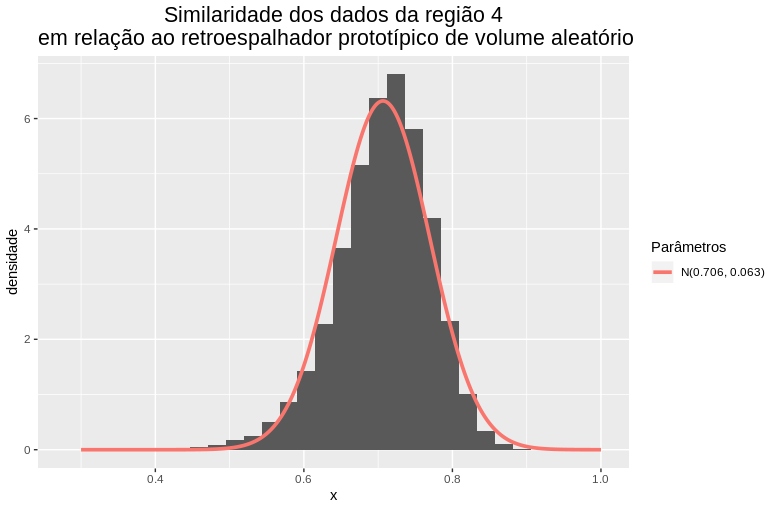
\includegraphics[width = \linewidth]{../../Images/Report_18_12_20/ponder_rv_region4.png}
    \caption{Região 4, Ponderosa Forest}
    \label{fig:pond_rv_r4}
\end{figure}

\begin{figure}[!h]
    \centering
    \vspace{0.1\linewidth}
    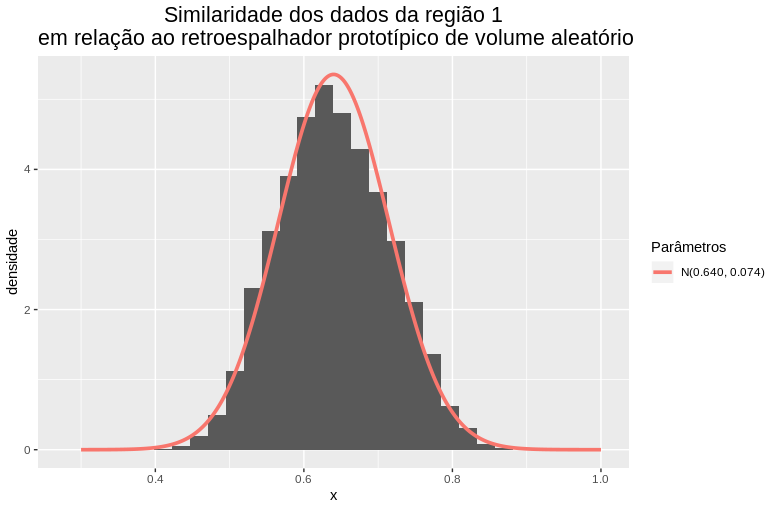
\includegraphics[width = \linewidth]{../../Images/Report_18_12_20/slum_rv_region1.png}
    \caption{Região 1, Slumgullion}
    \label{fig:slum_rv_r1}
\end{figure}

\begin{figure}[!h]
    \centering
    \vspace{0.1\linewidth}
    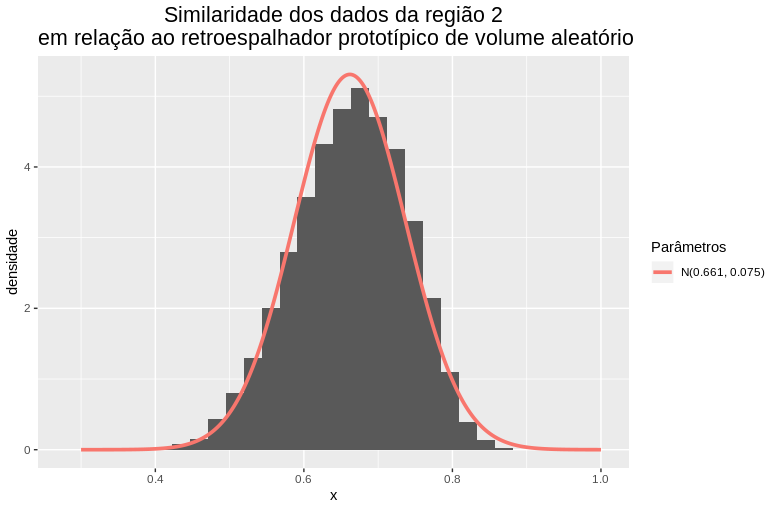
\includegraphics[width = \linewidth]{../../Images/Report_18_12_20/slum_rv_region2.png}
    \caption{Região 2, Slumgullion}
    \label{fig:slum_rv_r2}
\end{figure}

\begin{figure}[!h]
    \centering
    \vspace{0.1\linewidth}
    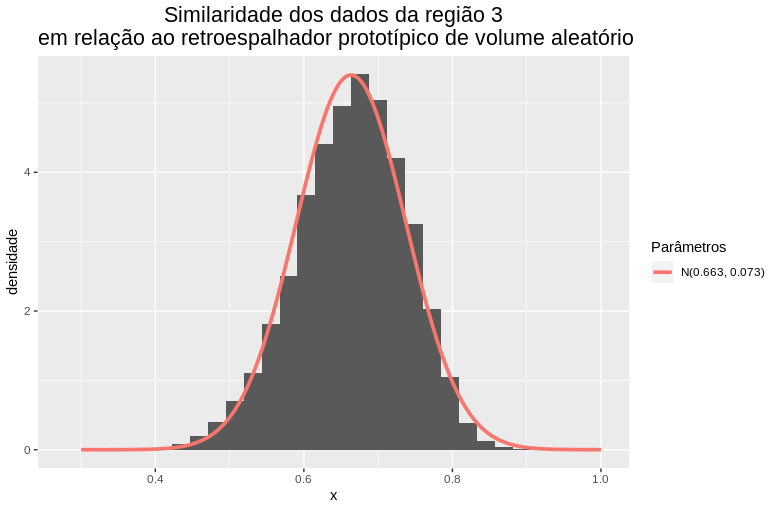
\includegraphics[width = \linewidth]{../../Images/Report_18_12_20/slum_rv_region3.png}
    \caption{Região 3, Slumgullion}
    \label{fig:slum_rv_r3}
\end{figure}
\newpage

As figuras \ref{fig:nd_r1}, \ref{fig:nd_r2}, \ref{fig:nd_r3}, \ref{fig:nd_r4} e \ref{fig:nd_r5} apresentam os histogramas das similaridades dos dados das regiões de vegetação da figura \ref{fig:img1} em relação ao retroespalhador prototípico \textit{narrow dihedral}. É observável o ajuste à distribuição Gama e a relativa proximidade entre os parâmetros estimados, com exceção da região 5.

\begin{figure}[!h]
    \centering
    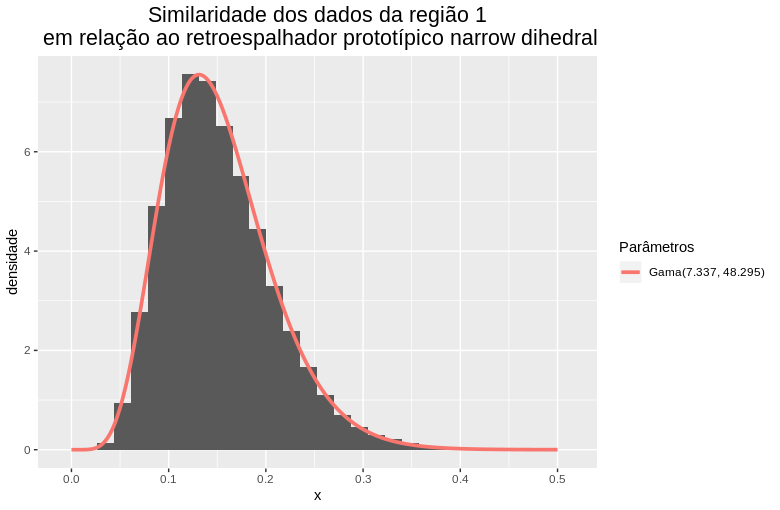
\includegraphics[width = \linewidth]{../../Images/Report_18_12_20/nd_region1.png}
    \caption{Região 1}
    \label{fig:nd_r1}
\end{figure}

\begin{figure}[!h]
    \centering
    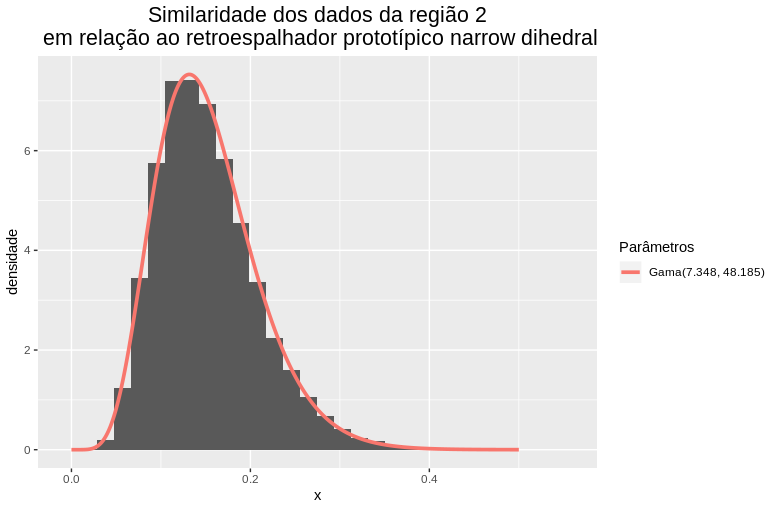
\includegraphics[width = \linewidth]{../../Images/Report_18_12_20/nd_region2.png}
    \caption{Região 2}
    \label{fig:nd_r2}
\end{figure}

\begin{figure}[!h]
    \centering
    \vspace{0.1\linewidth}
    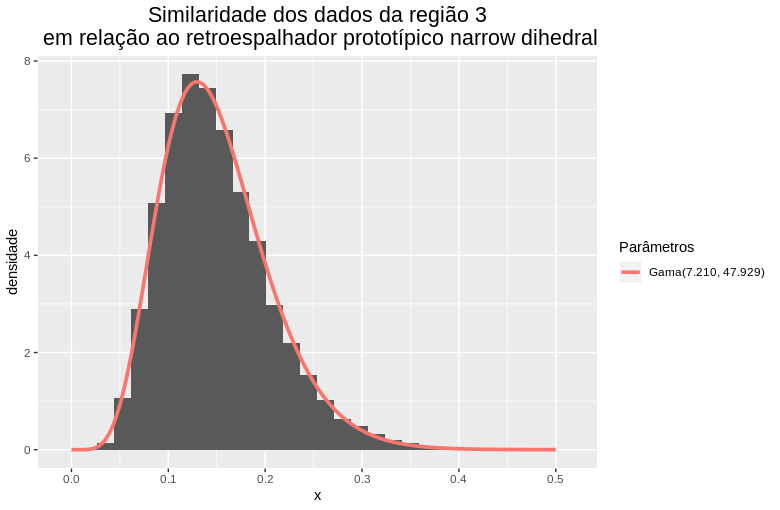
\includegraphics[width = \linewidth]{../../Images/Report_18_12_20/nd_region3.png}
    \caption{Região 3}
    \label{fig:nd_r3}
\end{figure}

\begin{figure}[!h]
    \centering
    \vspace{0.1\linewidth}
    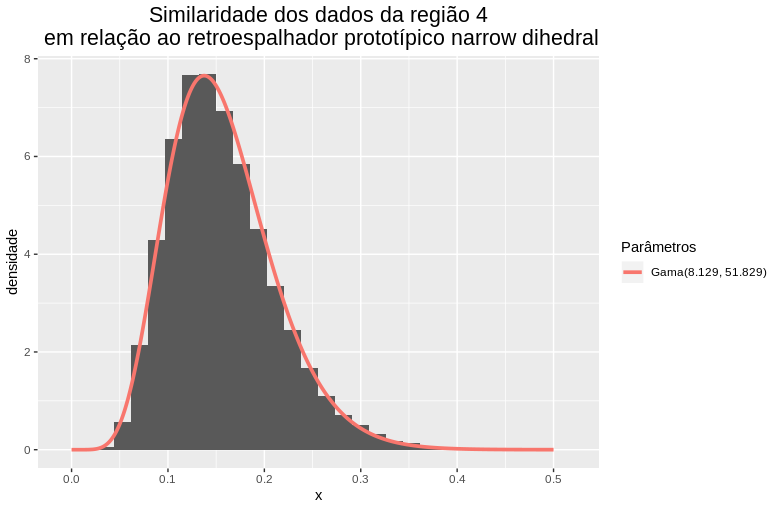
\includegraphics[width = \linewidth]{../../Images/Report_18_12_20/nd_region4.png}
    \caption{Região 4}
    \label{fig:nd_r4}
\end{figure}

\begin{figure}[!h]
    \centering
    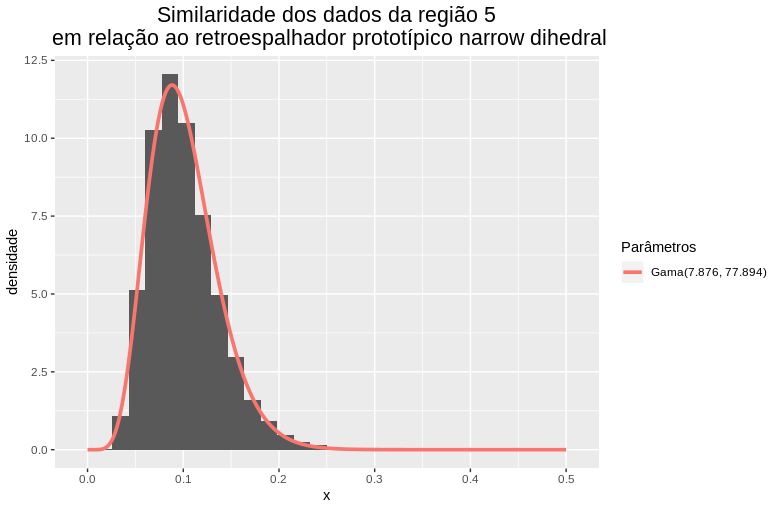
\includegraphics[width = \linewidth]{../../Images/Report_18_12_20/nd_region5.png}
    \caption{Região 5}
    \label{fig:nd_r5}
\end{figure}

As figuras \ref{fig:cy_r1}, \ref{fig:cy_r2}, \ref{fig:cy_r3}, \ref{fig:cy_r4} e \ref{fig:cy_r5} apresentam os histogramas das similaridades dos dados das regiões de vegetação da figura \ref{fig:img1} em relação ao retroespalhador prototípico \textit{cylinder}. É observável o ajuste à distribuição Normal e a relativa proximidade entre os parâmetros estimados.

\begin{figure}[!h]
    \centering
    \vspace{0.05\linewidth}
    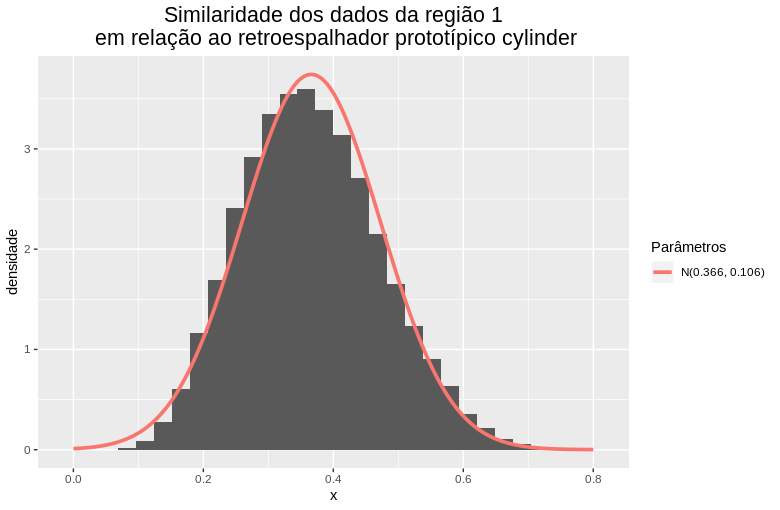
\includegraphics[width = \linewidth]{../../Images/Report_18_12_20/cy_region1.png}
    \caption{Região 1}
    \label{fig:cy_r1}
\end{figure}

\begin{figure}[!h]
    \centering
    \vspace{0.08\linewidth}
    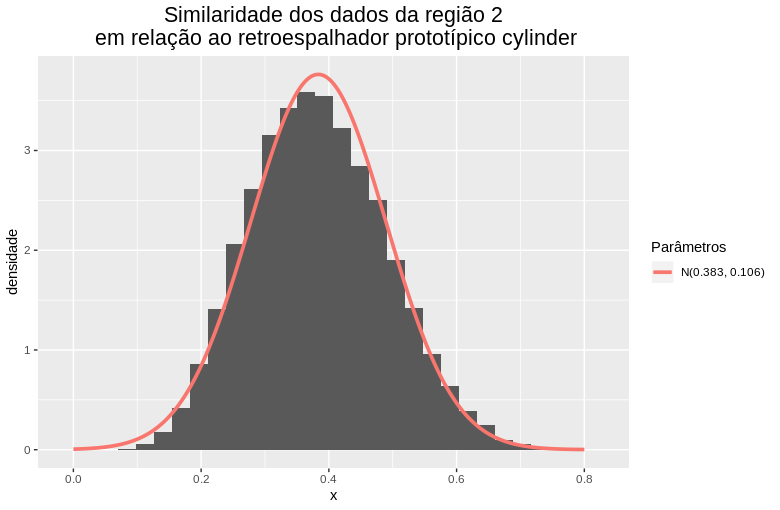
\includegraphics[width = \linewidth]{../../Images/Report_18_12_20/cy_region2.png}
    \caption{Região 2}
    \label{fig:cy_r2}
\end{figure}

\begin{figure}[!h]
    \centering
    \vspace{0.1\linewidth}
    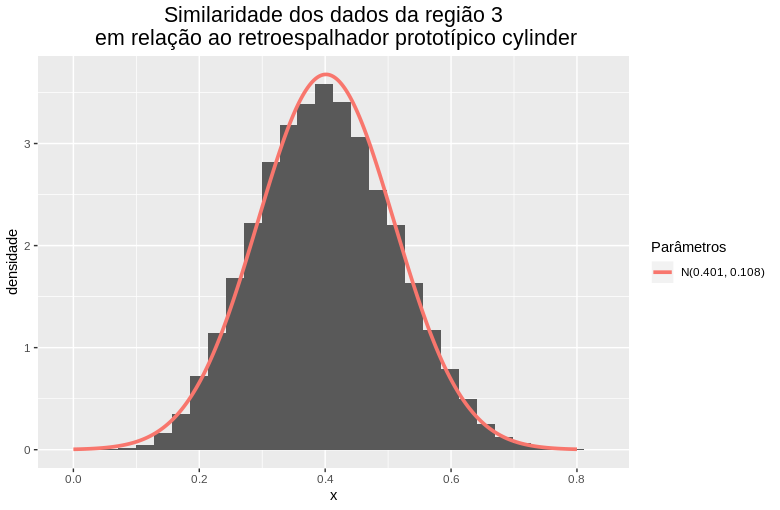
\includegraphics[width = \linewidth]{../../Images/Report_18_12_20/cy_region3.png}
    \caption{Região 3}
    \label{fig:cy_r3}
\end{figure}

\begin{figure}[!h]
    \centering
    \vspace{0.1\linewidth}
    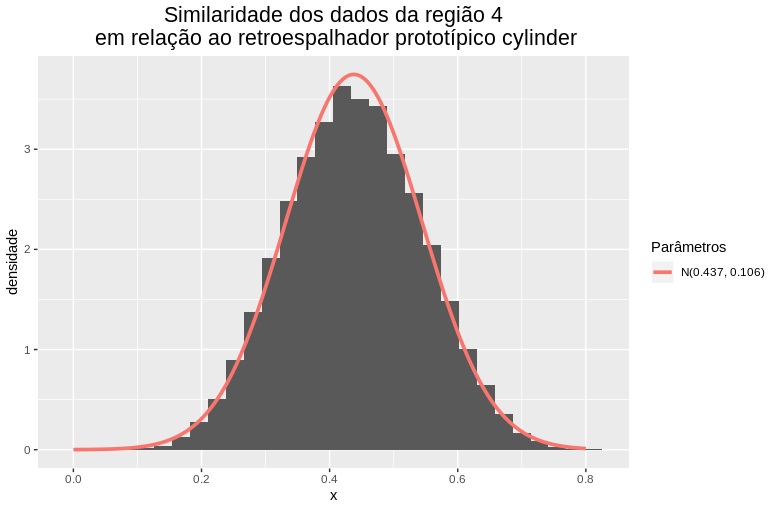
\includegraphics[width = \linewidth]{../../Images/Report_18_12_20/cy_region4.png}
    \caption{Região 4}
    \label{fig:cy_r4}
\end{figure}

\begin{figure}[!h]
    \centering
    \vspace{0.1\linewidth}
    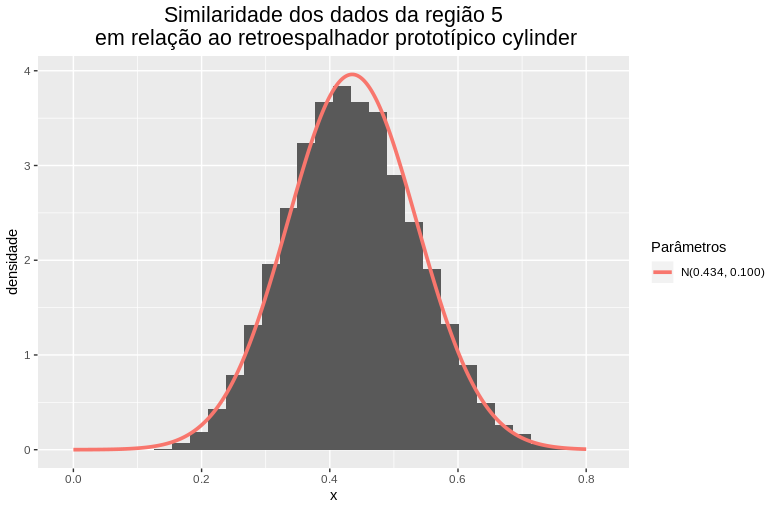
\includegraphics[width = \linewidth]{../../Images/Report_18_12_20/cy_region5.png}
    \caption{Região 5}
    \label{fig:cy_r5}
\end{figure}

As figuras \ref{fig:dip_r1}, \ref{fig:dip_r2}, \ref{fig:dip_r3}, \ref{fig:dip_r4} e \ref{fig:dip_r5} apresentam os histogramas das similaridades dos dados das regiões de vegetação da figura \ref{fig:img1} em relação ao retroespalhador prototípico \textit{dipole}. É observável o ajuste à distribuição Gama e a relativa proximidade entre os parâmetros estimados, com exceção do histograma da figura \ref{fig:dip_r5}.

\begin{figure}[!h]
    \centering
    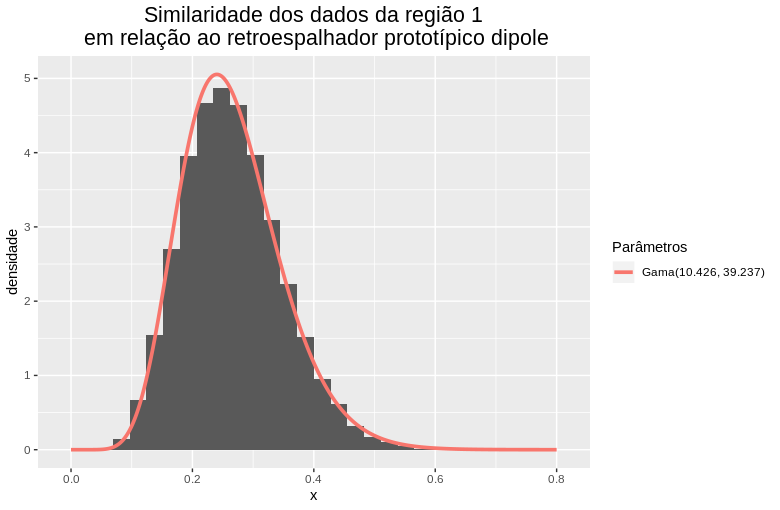
\includegraphics[width = \linewidth]{../../Images/Report_18_12_20/dip_region1.png}
    \caption{Região 1}
    \label{fig:dip_r1}
\end{figure}

\begin{figure}[!h]
    \centering
    \includegraphics[width = \linewidth]{../../Images/Report_18_12_20/dip_region2.png}
    \caption{Região 2}
    \label{fig:dip_r2}
\end{figure}

\begin{figure}[!h]
    \centering
    \vspace{0.1\linewidth}
    \includegraphics[width = \linewidth]{../../Images/Report_18_12_20/dip_region3.png}
    \caption{Região 3}
    \label{fig:dip_r3}
\end{figure}

\begin{figure}[!h]
    \centering
    \vspace{0.1\linewidth}
    \includegraphics[width = \linewidth]{../../Images/Report_18_12_20/dip_region4.png}
    \caption{Região 4}
    \label{fig:dip_r4}
\end{figure}

\begin{figure}[!h]
    \centering
    \includegraphics[width = \linewidth]{../../Images/Report_18_12_20/dip_region5.png}
    \caption{Região 5}
    \label{fig:dip_r5}
\end{figure}

As figuras \ref{fig:lh_r1}, \ref{fig:lh_r2}, \ref{fig:lh_r3}, \ref{fig:lh_r4} e \ref{fig:lh_r5} apresentam os histogramas das similaridades dos dados das regiões de vegetação da figura \ref{fig:img1} em relação ao retroespalhador prototípico \textit{left helix}. É observável o ajuste a distribuição Gama e a relativa proximidade entre os parâmetros estimados, com execeção do histograma da figura \ref{fig:lh_r5}.

\begin{figure}[!h]
    \centering
    \includegraphics[width = \linewidth]{../../Images/Report_18_12_20/lh_region1.png}
    \caption{Região 1}
    \label{fig:lh_r1}
\end{figure}

\begin{figure}[!h]
    \centering
    \vspace{0.1\linewidth}
    \includegraphics[width = \linewidth]{../../Images/Report_18_12_20/lh_region2.png}
    \caption{Região 2}
    \label{fig:lh_r2}
\end{figure}

\begin{figure}[!h]
    \centering
    \vspace{0.1\linewidth}
    \includegraphics[width = \linewidth]{../../Images/Report_18_12_20/lh_region3.png}
    \caption{Região 3}
    \label{fig:lh_r3}
\end{figure}

\begin{figure}[!h]
    \centering
    \vspace{0.10\linewidth}
    \includegraphics[width = \linewidth]{../../Images/Report_18_12_20/lh_region4.png}
    \caption{Região 4}
    \label{fig:lh_r4}
\end{figure}

\begin{figure}[!h]
    \centering
    \vspace{0.1\linewidth}
    \includegraphics[width = \linewidth]{../../Images/Report_18_12_20/lh_region5.png}
    \caption{Região 5}
    \label{fig:lh_r5}
\end{figure}

As figuras \ref{fig:rh_r1}, \ref{fig:rh_r2}, \ref{fig:rh_r3}, \ref{fig:rh_r4} e \ref{fig:rh_r5} apresentam os histogramas das similaridades dos dados das regiões de vegetação da figura \ref{fig:img1} em relação ao retroespalhador prototípico \textit{right helix}. É observável o ajuste a distribuição Gama e a relativa proximidade entre os parâmetros estimados, com execeção do histograma da figura \ref{fig:rh_r5}.

\begin{figure}[!h]
    \centering
    \includegraphics[width = \linewidth]{../../Images/Report_18_12_20/rh_region1.png}
    \caption{Região 1}
    \label{fig:rh_r1}
\end{figure}

\begin{figure}[!h]
    \centering
    \includegraphics[width = \linewidth]{../../Images/Report_18_12_20/rh_region2.png}
    \caption{Região 2}
    \label{fig:rh_r2}
\end{figure}

\begin{figure}[!h]
    \centering
    \vspace{0.1\linewidth}
    \includegraphics[width = \linewidth]{../../Images/Report_18_12_20/rh_region3.png}
    \caption{Região 3}
    \label{fig:rh_r3}
\end{figure}

\begin{figure}[!h]
    \centering
    \vspace{0.1\linewidth}
    \includegraphics[width = \linewidth]{../../Images/Report_18_12_20/rh_region4.png}
    \caption{Região 4}
    \label{fig:rh_r4}
\end{figure}

\begin{figure}[!h]
    \centering
    \includegraphics[width = \linewidth]{../../Images/Report_18_12_20/rh_region5.png}
    \caption{Região 5}
    \label{fig:rh_r5}
\end{figure}

As figuras \ref{fig:pwv_r1}, \ref{fig:pwv_r2}, \ref{fig:pwv_r3}, \ref{fig:pwv_r4} e \ref{fig:pwv_r5} apresentam os histogramas das similaridades dos dados das regiões de vegetação da figura \ref{fig:img1} em relação ao retroespalhador prototípico \textit{+1/4-wave}. É observável o ajuste a distribuição Gama e a relativa proximidade entre os parâmetros estimados, com execeção do histograma da figura \ref{fig:pwv_r5}.

\begin{figure}[!h]
    \centering
    \vspace{0.05\linewidth}
    \includegraphics[width = \linewidth]{../../Images/Report_18_12_20/pwv_region1.png}
    \caption{Região 1}
    \label{fig:pwv_r1}
\end{figure}

\begin{figure}[!h]
    \centering
    \vspace{0.07\linewidth}
    \includegraphics[width = \linewidth]{../../Images/Report_18_12_20/pwv_region2.png}
    \caption{Região 2}
    \label{fig:pwv_r2}
\end{figure}

\begin{figure}[!h]
    \centering
    \vspace{0.1\linewidth}
    \includegraphics[width = \linewidth]{../../Images/Report_18_12_20/pwv_region3.png}
    \caption{Região 3}
    \label{fig:pwv_r3}
\end{figure}

\begin{figure}[!h]
    \centering
    \vspace{0.1\linewidth}
    \includegraphics[width = \linewidth]{../../Images/Report_18_12_20/pwv_region4.png}
    \caption{Região 4}
    \label{fig:pwv_r4}
\end{figure}

\begin{figure}[!h]
    \centering
    \vspace{0.1\linewidth}
    \includegraphics[width = \linewidth]{../../Images/Report_18_12_20/pwv_region5.png}
    \caption{Região 5}
    \label{fig:pwv_r5}
\end{figure}

As figuras \ref{fig:nwv_r1}, \ref{fig:nwv_r2}, \ref{fig:nwv_r3}, \ref{fig:nwv_r4} e \ref{fig:nwv_r5} apresentam os histogramas das similaridades dos dados das regiões de vegetação da figura \ref{fig:img1} em relação ao retroespalhador prototípico \textit{-1/4-wave}. É observável o ajuste a distribuição Gama e a relativa proximidade entre os parâmetros estimados, com execeção do histograma da figura \ref{fig:nwv_r5}.

\begin{figure}[!h]
    \centering
    \includegraphics[width = \linewidth]{../../Images/Report_18_12_20/nwv_region1.png}
    \caption{Região 1}
    \label{fig:nwv_r1}
\end{figure}

\begin{figure}[!h]
    \centering
    \includegraphics[width = \linewidth]{../../Images/Report_18_12_20/nwv_region2.png}
    \caption{Região 2}
    \label{fig:nwv_r2}
\end{figure}

\begin{figure}[!h]
    \centering
    \vspace{0.1\linewidth}
    \includegraphics[width = \linewidth]{../../Images/Report_18_12_20/nwv_region3.png}
    \caption{Região 3}
    \label{fig:nwv_r3}
\end{figure}

\begin{figure}[!h]
    \centering
    \vspace{0.1\linewidth}
    \includegraphics[width = \linewidth]{../../Images/Report_18_12_20/nwv_region4.png}
    \caption{Região 4}
    \label{fig:nwv_r4}
\end{figure}

\begin{figure}[!h]
    \centering
    \includegraphics[width = \linewidth]{../../Images/Report_18_12_20/nwv_region5.png}
    \caption{Região 5}
    \label{fig:nwv_r5}
\end{figure}

As figuras \ref{fig:tri_r6}, \ref{fig:tri_r7} e \ref{fig:tri_r8} apresentam os histogramas das similaridades dos dados das regiões 6 à 8 da figura \ref{fig:img1}, as quais são regiões de solo exposto, em relação ao retroespalhador prototípico \textit{trihedral}. Observemos que há uma considerável variabilidade nos parâmetros e que não houve ajuste à distribuição Gama no histograma da figura \ref{fig:tri_r6}. 

\begin{figure}[!h]
    \centering
    \includegraphics[width = 0.95\linewidth]{../../Images/Report_18_12_17/tri_region6.png}
    \caption{Região 6, Guatemala}
    \label{fig:tri_r6}
\end{figure}

\begin{figure}[!h]
    \centering
    \vspace{0.1\linewidth}
    \includegraphics[width = 0.95\linewidth]{../../Images/Report_18_12_17/tri_region7.png}
    \caption{Região 7, Guatemala}
    \label{fig:tri_r7}
\end{figure}

\begin{figure}[!h]
    \centering    
    \vspace{0.15\linewidth}
    \includegraphics[width = 0.95\linewidth]{../../Images/Report_18_12_17/tri_region8.png}
    \caption{Região 8, Guatemala}
    \label{fig:tri_r8}
\end{figure}

As figuras \ref{fig:di_r6}, \ref{fig:di_r7} e \ref{fig:di_r8} apresentam os histogramas das similaridades dos dados das regiões 6 à 8 referentes à figura \ref{fig:img1} em relação ao retroespalhador prototípico \textit{dihedral}. Embora haja o ajuste a distribuição Gama, também há considerável variabilidade nos parâmetros.

\begin{figure}[!h]
    \centering
    \includegraphics[width = 0.95\linewidth]{../../Images/Report_18_12_17/di_region6.png}
    \caption{Região 6, Guatemala}
    \label{fig:di_r6}
\end{figure}

\begin{figure}[!h]
    \centering
    \vspace{0.05\linewidth}
    \includegraphics[width = 0.95\linewidth]{../../Images/Report_18_12_17/di_region7.png}
    \caption{Região 7, Guatemala}
    \label{fig:di_r7}
\end{figure}

\begin{figure}[!h]
    \centering    
    \includegraphics[width = 0.95\linewidth]{../../Images/Report_18_12_17/di_region8.png}
    \caption{Região 8, Guatemala}
    \label{fig:di_r8}
\end{figure}

As figuras \ref{fig:rv_r6}, \ref{fig:rv_r7} e \ref{fig:rv_r8} apresentam os histogramas das similaridades dos dados das regiões 6 à 8 referentes à figura \ref{fig:img1} em relação ao retroespalhador prototípico de \textit{random volume}. Observemos que não houve ajuste dos histogramas à distribuição Gama.

\begin{figure}[!h]
    \centering
    \includegraphics[width = 0.95\linewidth]{../../Images/Report_18_12_17/rv_region6.png}
    \caption{Região 6, Guatemala}
    \label{fig:rv_r6}
\end{figure}

\begin{figure}[!h]
    \centering
    \vspace{0.05\linewidth}
    \includegraphics[width = 0.95\linewidth]{../../Images/Report_18_12_17/rv_region7.png}
    \caption{Região 7, Guatemala}
    \label{fig:rv_r7}
\end{figure}

\begin{figure}[!h]
    \centering    
    \vspace{0.1\linewidth}
    \includegraphics[width = 0.95\linewidth]{../../Images/Report_18_12_17/rv_region8.png}
    \caption{Região 8, Guatemala}
    \label{fig:rv_r8}
\end{figure}

\newpage

\bibliographystyle{abntex2-alf}
\bibliography{Bibliography/ref_18_12_17}

\end{document}
